\paragraph{Allgemein}
Für die Tassenerkennung wurden keinerlei ROS Pakete verwendet. Stattdessen wurden die einzelnen Komponenten in Python selbst implementiert. Die am häufigsten zur Hilfe genommenen Bibliotheken sind unter anderem:
\begin{itemize}
\item NumPy (Effizienter Umgang mit Matrizen und Vektoren)
\item scikit-image (Bildverarbeitung)
\item scikit-learn (Algorithmen für Maschinelles Lernen)
\item Keras (High-level API für die Erstellung von Neuronalen Netzen)
\item Matplotlib (Visualisierung)
\end{itemize}

\paragraph{Detektion der Tasse in den Bilddaten}
Für die Detektion der Tasse in den Bilddaten wurden eine Reihe von Ansätzen getestet, bevor die finale Lösung feststand.

Zunächst war der Plan die Tasse mittels eines Fully Convolutional Neural Network aus den Bilddaten zu segmentieren. Als Basisstruktur wurde hierfür die Architektur des Resnet50 Netzes verwendet. Die Eingabe für das Netz stellt ein RGB Bild dar und es liefert als Ausgabe zwei Feature Maps, welche die Wahrscheinlichkeiten für die Zugehörigkeiten der Pixel des Eingabebildes zu den Klassen \glqq Tasse\grqq bzw. \glqq Keine Tasse\grqq enthalten. Trainiert wurde auf den Microsoft COCO Datensatz unter Nutzung von GPU Kapazitäten bei Amazon Webservices. Der Ansatz wurde letztendlich verworfen, da es sich herausstellte dass das Netz zu überdimensioniert für die Segmentierung einer Klasse aus einem RGB Datensatz ist und nicht genügend Trainingsdaten zur Verfügung standen.

Der zweite getestete Ansatz basierte auf der Segmentierung des Bildes in eine Menge von Segmenten sowie einer Klassifizierung durch ein Neuronales Netz. Das Bild wird hierfür zunächst mittels des SLIC Algorithmus in eine Menge von Segmenten zerlegt. Diese Segmente werden dann unter Einbeziehung eines gewissen Kontextfensters dem Neuronalen Netz zur Klassifikation übergeben. Jedem Segment wird entweder als \glqq Tasse\grqq oder \glqq Keine Tasse\grqq klassifiziert. Das Ergebnis einer Vorhersage mit dem beschriebenen Algorithmus ist in Abbildung \ref{fig:patches_prediction_result} abgebildet.

\begin{figure}
    \centering
    \begin{minipage}{0.45\textwidth}
        \centering
        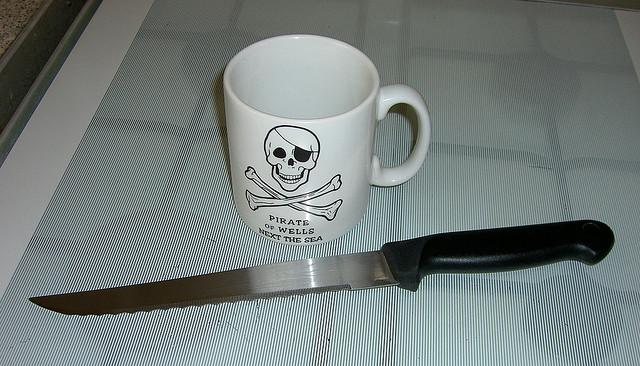
\includegraphics[width=0.9\textwidth]{images/cup_patches.jpg} % first figure itself
        \caption{Eingabe für das Neuronale Netz zur Segment Klassifikation \label{fig:patches_prediction}}
    \end{minipage}\hfill
    \begin{minipage}{0.48\textwidth}
        \centering
        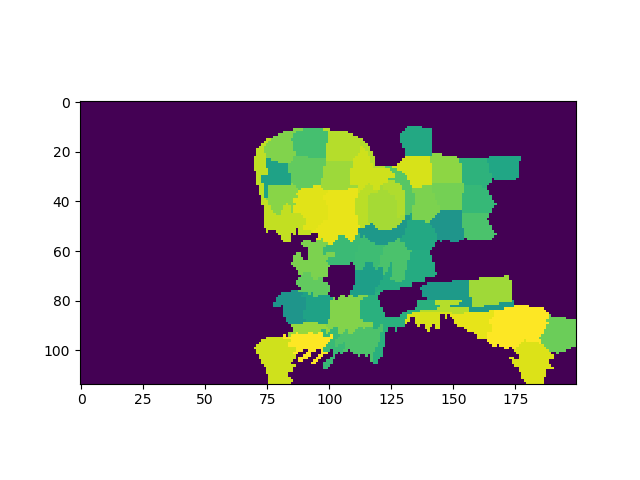
\includegraphics[width=0.9\textwidth]{images/cup_patches_prediction.png} % second figure itself
        \caption{Vom Netz ausgegebene Wahrscheinlichkeiten \label{fig:patches_prediction_result}}
    \end{minipage}
\end{figure}

Der dritte gewählte Ansatz wurde letztendlich auch in das fertige System übernommen und basiert auf einer SVM welche Bildsegmente, die mithilfe eines Sliding Window Ansatzes gewonnen werden klassifiziert. Details zu diesem Ansatz werden im Abschnitt \ref{4-1-1_gesamtsystem_bilderkennung_tassenerkennung} näher erläutert.

Neben den selbst implementierten Ansätzen wurde außerdem das YOLO Real-Time Object Detection System getestet. Hierbei handelt es sich im wesentlichen um ein vortrainiertes Neuronales Netz, welches in der Lage ist eine Vielzahl an Objektklassen zu detektieren (siehe auch \ref{fig:yolo}). Das System erwies sich hinsichtlich Geschwindigkeit und Genauigkeit als durchaus geeignet, jedoch haben wir uns dennoch dazu entschieden unsere eigenen Ansätze zu verwirklichen.

\begin{figure}
\centering
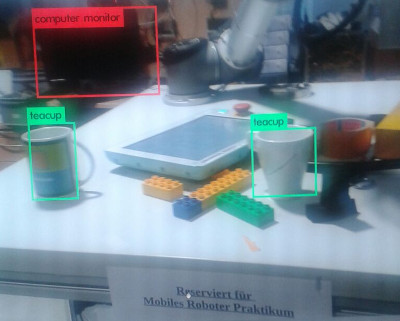
\includegraphics[scale=0.5]{./images/yolo.jpeg}
\caption{Erkennung der Tasse in der Szene Mithilfe von Yolo \label{fig:yolo}}
\end{figure}

\paragraph{Segmentierung der Tasse in der Punktwolke}
Nachdem die Tasse in den Bilddaten detektiert wurde wird sie mittels eines Clustering Algorithmus aus den Bilddaten segmentiert. Hierbei traten keinerlei Komplikationen auf. Der Ansatz wird ebenfalls in \ref{4-1-1_gesamtsystem_bilderkennung_tassenerkennung} beschrieben.

\paragraph{Erkennung der Tassenorientierung}
Hier wurden zwei verschiedene Ansätze implementiert wovon letztendlich einer für das finale System ausgewählt wurde. Der erste Ansatz basiert auf dem RANSAC Algorithmus. Zunächst wird die Punktwolke der Tasse auf die x-y-Ebene projiziert und deren Zentrum bestimmt. Anschließend wird in jeder Iteration des Ransac Algorithmus ein zufälliger Punkt ausgewählt und eine Linie durch selbigen und das Zentrum der Tasse gelegt. Es wird die Konfiguration mit den meisten Inliern als Richtung des Tassengriffs ausgewählt. Es stellte sich hierbei heraus, dass die zum Tassengriff gehörigen Punkte im Vergleich zu den restlichen Punkten so wenig ins Gewicht fallen dass so keine zuverlässige Schätzung möglich war.
Der zweite Ansatz basiert auf dem Local Outlier Factor Schätzer und erwies sich als deutlich robuster als der zuvor beschriebene Ansatz. Er wird in \ref{4-1-1_gesamtsystem_bilderkennung_tassenerkennung} näher beschrieben.